\iffalse
TODO Dit moet verder in detail worden beschreven
\fi

\chapter{Proof of Concept}
\label{ch:poc}

\section{Conway's Game of Life}
\label{sec:gool}

\textit{Conway's Game of Life} bevat simpele regels die toelaten om een simulatie makkelijk te implementeren, de enige complexiteit komt voort uit de schaal waarop de simulatie wordt uitgevoerd. Deze \textit{zero-player game} heeft namelijk geen begrenzing waarop het kan worden gespeeld. Dit wilt zeggen dat tot zover de rekenkracht het toestaat de simulatie op een oneindig grote schaal kan worden uitgevoerd. Verder betekent dit ook dat, samen met andere benodigdheden zoals logische poorten (\textit{AND, OR, NOT}) en het gebruik van signalen door middel van \textit{Gliders}, het mogelijk is om eender welk complex programma te simuleren, en ook \textit{Conway's Game of Life} zelf.

\bigbreak{}

De simpele regels van \textit{Life} zijn als volgt:
\begin{enumerate}
    \item Elke levende cel met minder dan twee buren sterft, als door onderbevolking.
    \item Elke levende cel met twee of drie buren blijft in leven tot de volgende generatie.
    \item Elke levende cel met meer dan drie buren sterft, als door overbevolking.
    \item Elke dode cel met precies drie buren in leven komt tot leven, als door reproductie.
\end{enumerate}


\break{}

Om de rekenkundige en grafische kant te representeren in een simpele implementatie werd deze simulatie geprogrammeerd met \textit{WebGPU}. Dit concept werd uitgevoerd op basis van de \textit{codelab} die beschikbaar werd gesteld door \textcite{google2023}. Hierdoor kan op een interactieve manier de werking van \textit{WGSL} worden aangeleerd zonder dat de nood bestaat om extreem complexe zaken te hoeven uit te werken.

\bigbreak{}

Afbeelding \ref{fig:Conway's Game of Life} geeft de \textit{Conway's Game of Life} implementatie weer en hoe deze beschikbaar is op \href{https://gool.qwict.com}{gool.qwict.com}.

\begin{figure}
    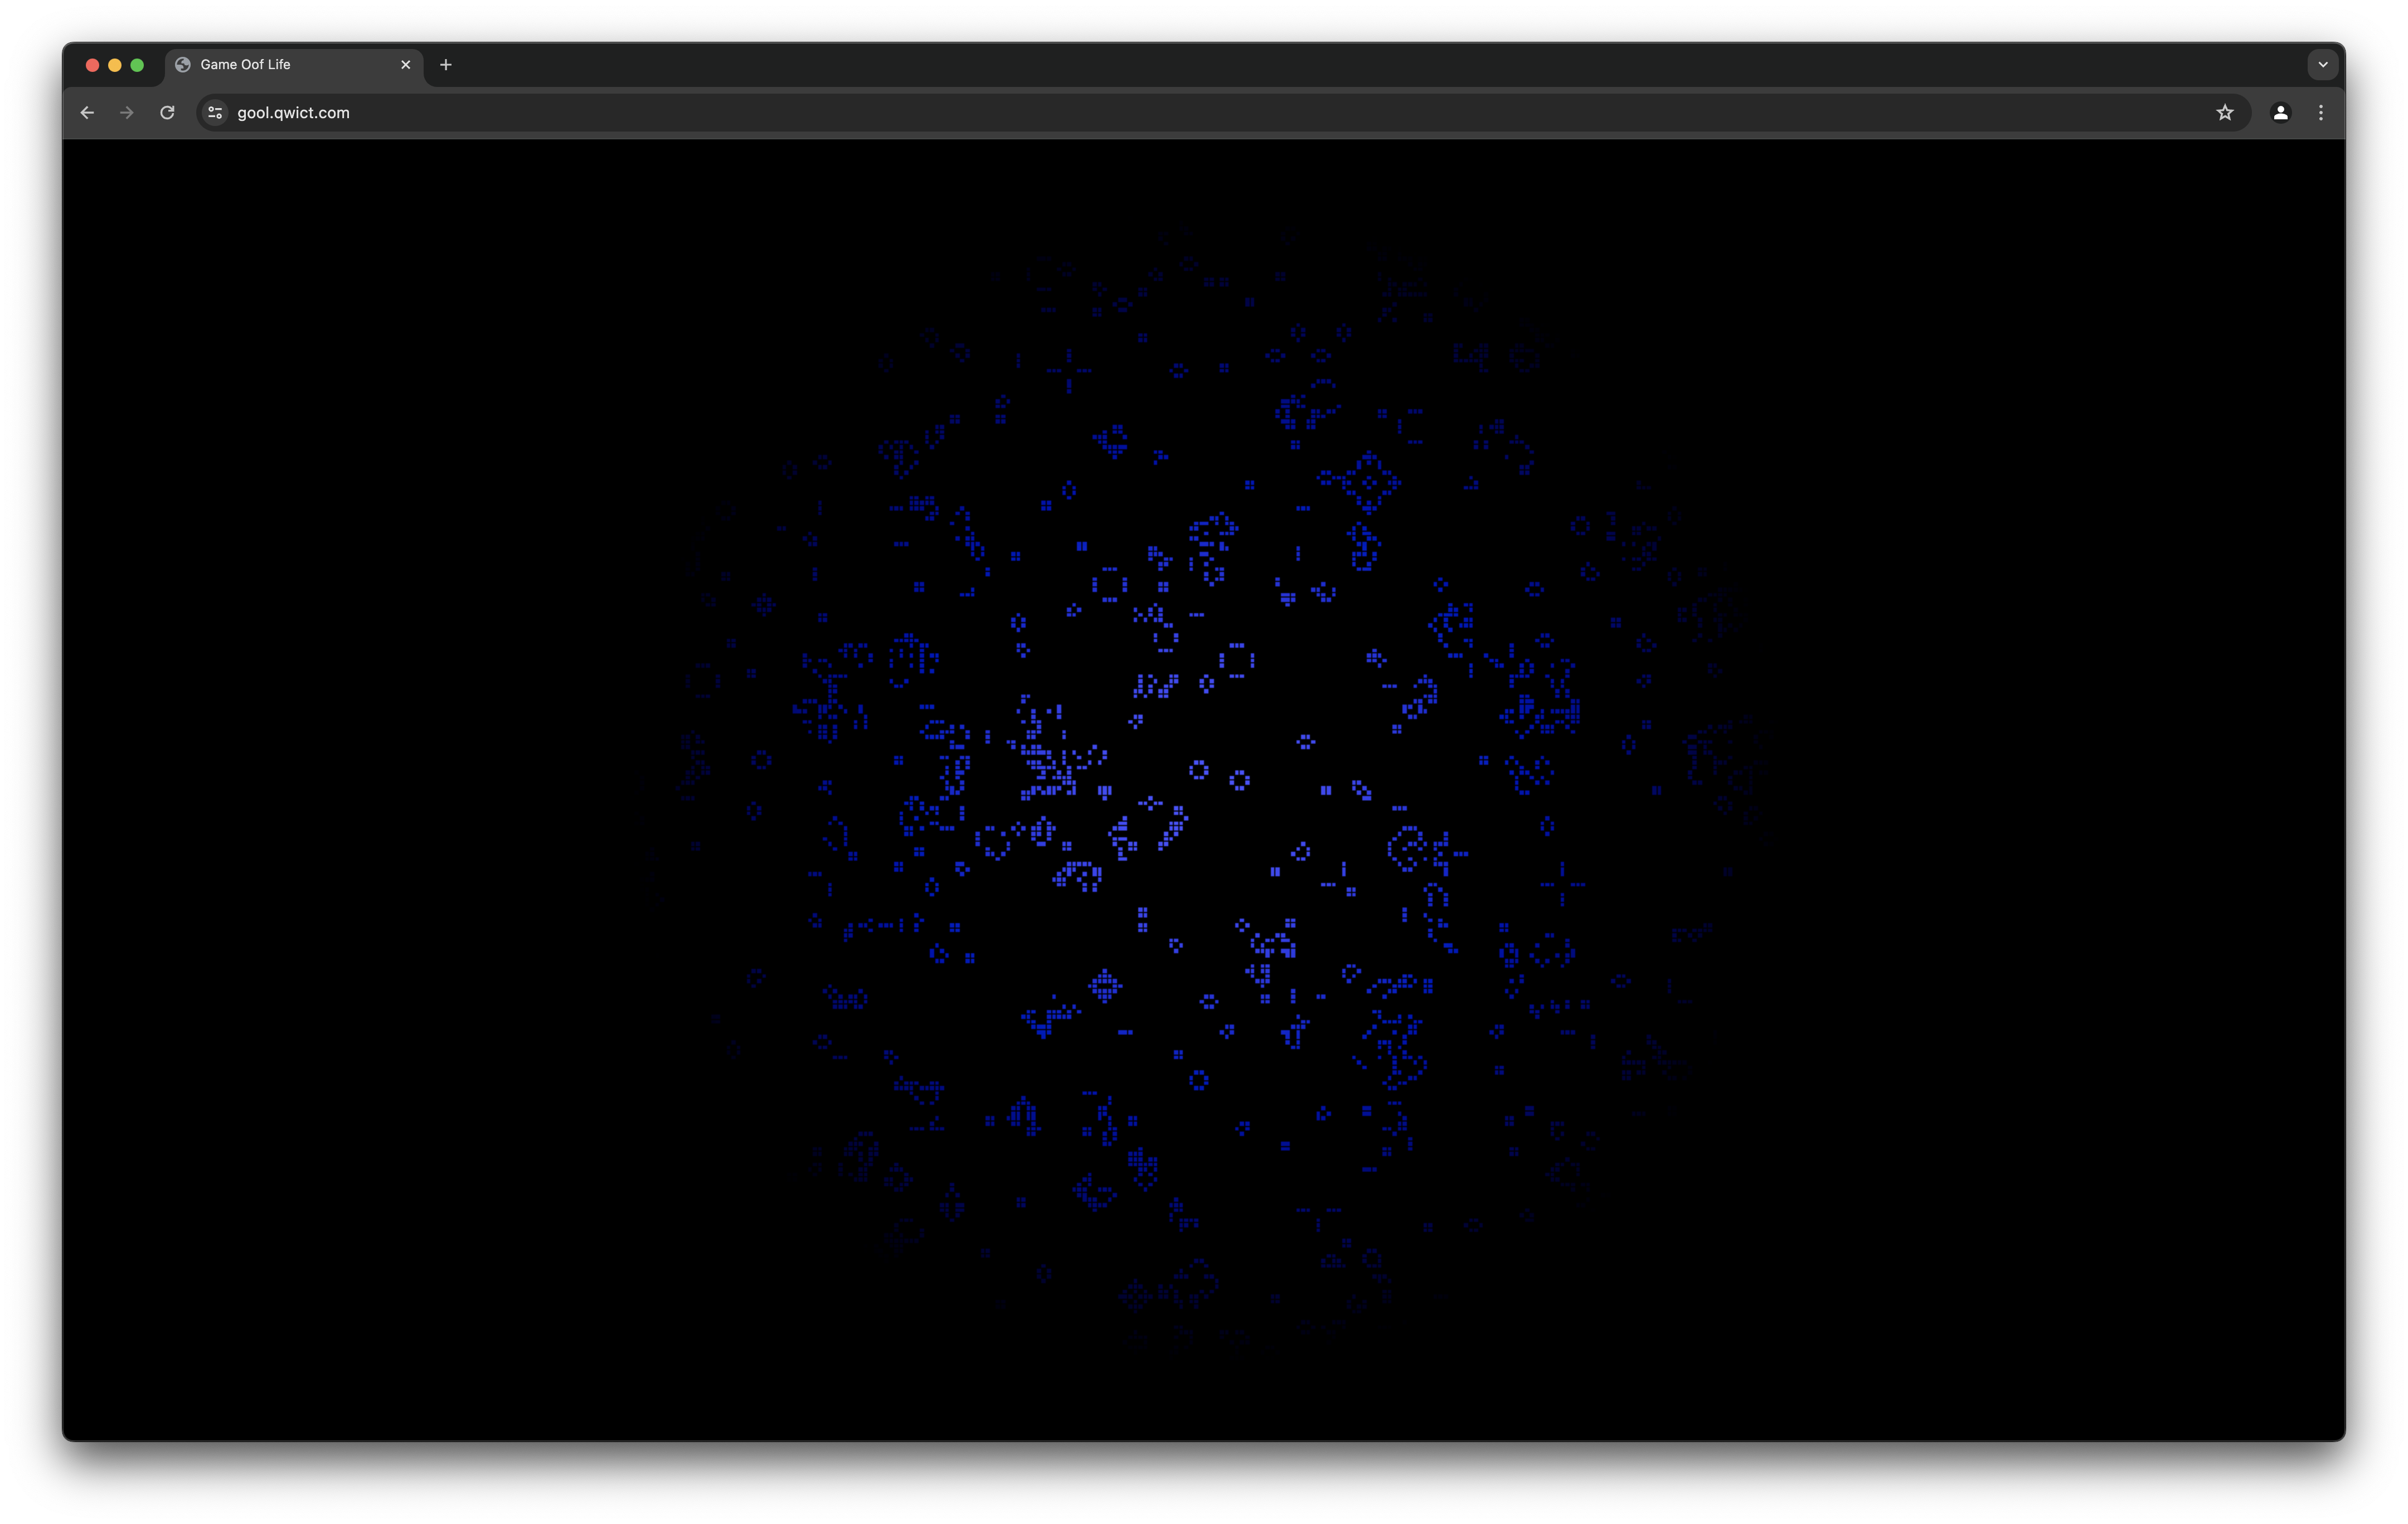
\includegraphics[width=\linewidth]{gool.png}
    \caption[Conway's \textit{Game of Life} implementatie~\autocite{google2023, Qwict2024}]{
        Conway's \textit{Game of Life} implementatie beschikbaar op \href{https://gool.qwict.com}{gool.qwict.com}. De broncode is beschikbaar op \href{https://github.com/qwict/GoolWebGPU}{GitHub.com/Qwict/GoolWebGPU}~\autocite{google2023, Qwict2024}.
    }
    \label{fig:Conway's Game of Life}
\end{figure}

\section{web-llm}
\label{sec:chatgpu}

Een implementatie van kunstmatige intelligentie in de browser werd verwezenlijkt door een voorbeeld van \textcite{mlcai2023} aan te passen en hierna te implementeren op eigen server apparatuur~\autocite{Qwict2024a}.

\bigbreak{}

De simpliciteit van deze implementatie toont aan dat het inzetten van open source modellen in combinatie met frameworks geen grote uitdaging hoeft te zijn voor kleinschalige software. Dit maakt \textit{WebGPU} een geschikt alternatief voor het gebruik van \textit{Web APIs} die kunstmatige intelligentie voorzien als een dienst.

\bigbreak{}

Afbeelding \ref{fig:Implementatie web-llm} geeft de \textit{web-llm} implementatie weer hoe deze beschikbaar is op \href{https://chatgpu.qwict.com}{chatgpu.qwict.com}~\autocite{Qwict2024a}.

\begin{figure}
    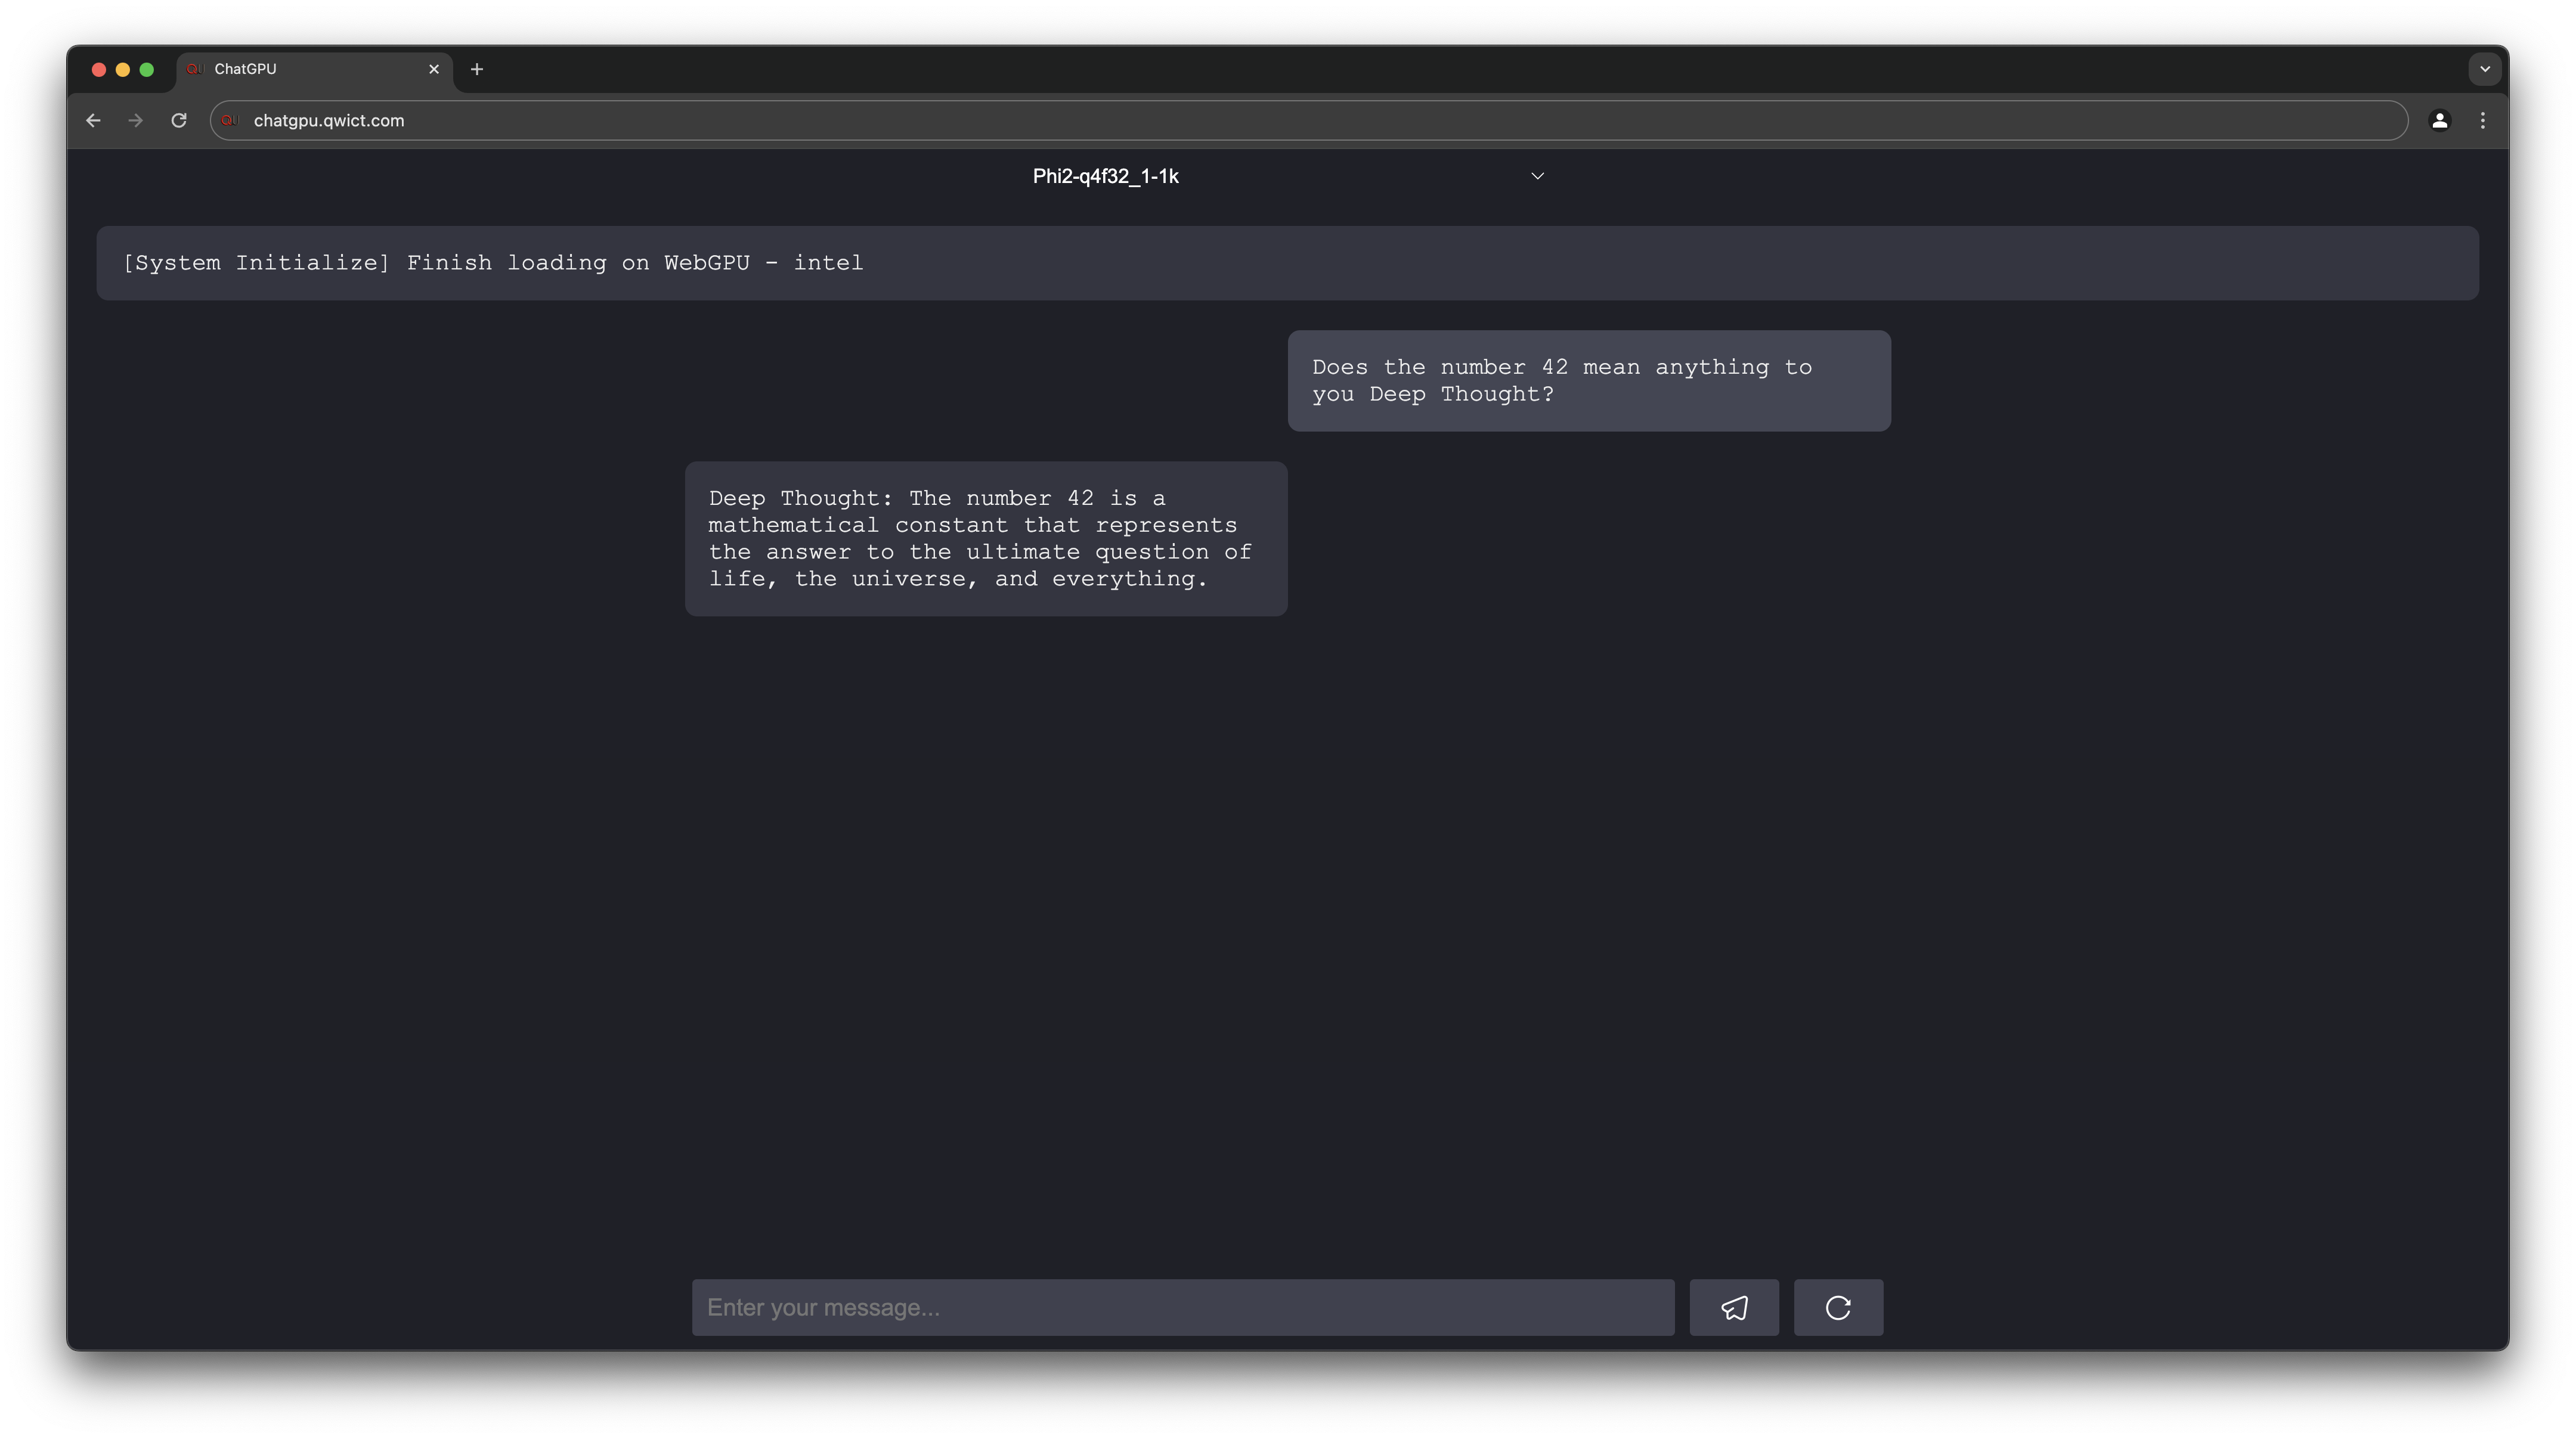
\includegraphics[width=\linewidth]{chatgpu.png}
    \caption[Implementatie web-llm~\autocite{mlcai2023, Qwict2024a}]{
        Implementatie web-llm beschikbaar op \href{https://chatgpu.qwict.com}{chatgpu.qwict.com}. De broncode is beschikbaar op \href{https://github.com/qwict/chatgpu}{GitHub.com/Qwict/ChatGPU}~\autocite{mlcai2023, Qwict2024a}.
    }
    \label{fig:Implementatie web-llm}
\end{figure}